% Options for packages loaded elsewhere
\PassOptionsToPackage{unicode}{hyperref}
\PassOptionsToPackage{hyphens}{url}
%
\documentclass[
]{book}
\usepackage{amsmath,amssymb}
\usepackage{lmodern}
\usepackage{ifxetex,ifluatex}
\ifnum 0\ifxetex 1\fi\ifluatex 1\fi=0 % if pdftex
  \usepackage[T1]{fontenc}
  \usepackage[utf8]{inputenc}
  \usepackage{textcomp} % provide euro and other symbols
\else % if luatex or xetex
  \usepackage{unicode-math}
  \defaultfontfeatures{Scale=MatchLowercase}
  \defaultfontfeatures[\rmfamily]{Ligatures=TeX,Scale=1}
\fi
% Use upquote if available, for straight quotes in verbatim environments
\IfFileExists{upquote.sty}{\usepackage{upquote}}{}
\IfFileExists{microtype.sty}{% use microtype if available
  \usepackage[]{microtype}
  \UseMicrotypeSet[protrusion]{basicmath} % disable protrusion for tt fonts
}{}
\makeatletter
\@ifundefined{KOMAClassName}{% if non-KOMA class
  \IfFileExists{parskip.sty}{%
    \usepackage{parskip}
  }{% else
    \setlength{\parindent}{0pt}
    \setlength{\parskip}{6pt plus 2pt minus 1pt}}
}{% if KOMA class
  \KOMAoptions{parskip=half}}
\makeatother
\usepackage{xcolor}
\IfFileExists{xurl.sty}{\usepackage{xurl}}{} % add URL line breaks if available
\IfFileExists{bookmark.sty}{\usepackage{bookmark}}{\usepackage{hyperref}}
\hypersetup{
  pdftitle={CPS in Japan},
  pdfauthor={Keisuke Kawata},
  hidelinks,
  pdfcreator={LaTeX via pandoc}}
\urlstyle{same} % disable monospaced font for URLs
\usepackage{longtable,booktabs,array}
\usepackage{calc} % for calculating minipage widths
% Correct order of tables after \paragraph or \subparagraph
\usepackage{etoolbox}
\makeatletter
\patchcmd\longtable{\par}{\if@noskipsec\mbox{}\fi\par}{}{}
\makeatother
% Allow footnotes in longtable head/foot
\IfFileExists{footnotehyper.sty}{\usepackage{footnotehyper}}{\usepackage{footnote}}
\makesavenoteenv{longtable}
\usepackage{graphicx}
\makeatletter
\def\maxwidth{\ifdim\Gin@nat@width>\linewidth\linewidth\else\Gin@nat@width\fi}
\def\maxheight{\ifdim\Gin@nat@height>\textheight\textheight\else\Gin@nat@height\fi}
\makeatother
% Scale images if necessary, so that they will not overflow the page
% margins by default, and it is still possible to overwrite the defaults
% using explicit options in \includegraphics[width, height, ...]{}
\setkeys{Gin}{width=\maxwidth,height=\maxheight,keepaspectratio}
% Set default figure placement to htbp
\makeatletter
\def\fps@figure{htbp}
\makeatother
\setlength{\emergencystretch}{3em} % prevent overfull lines
\providecommand{\tightlist}{%
  \setlength{\itemsep}{0pt}\setlength{\parskip}{0pt}}
\setcounter{secnumdepth}{5}
\usepackage{booktabs}
\ifluatex
  \usepackage{selnolig}  % disable illegal ligatures
\fi
\usepackage[]{natbib}
\bibliographystyle{apalike}

\title{CPS in Japan}
\author{Keisuke Kawata}
\date{2021-06-30}

\begin{document}
\maketitle

{
\setcounter{tocdepth}{1}
\tableofcontents
}
\hypertarget{summary}{%
\chapter{Summary}\label{summary}}

\begin{itemize}
\tightlist
\item
  Use the \href{https://www.stat.go.jp/english/data/roudou/index.html}{Labor force survey}, which is open-access and includes similar variables as the current population survey in U.S.
\end{itemize}

\hypertarget{simple-description-long-run}{%
\chapter{Simple description: Long-run}\label{simple-description-long-run}}

\begin{itemize}
\tightlist
\item
  Describe labor market after 1969.
\end{itemize}

\hypertarget{environment}{%
\section{Environment}\label{environment}}

\hypertarget{data}{%
\section{Data}\label{data}}

\hypertarget{employment-rate}{%
\section{Employment rate}\label{employment-rate}}

\begin{itemize}
\tightlist
\item
  Report \(e_{g,m,y} = \frac{Employment_{g,m,y}}{Population_{g,m,y}}\), where \(Employment_{g,m,y}\) and \(Population_{g,m,y}\) are numbers of employment and population over 15 years old in month \(m\), year \(y\) and gender group \(g\), respectively.
\end{itemize}

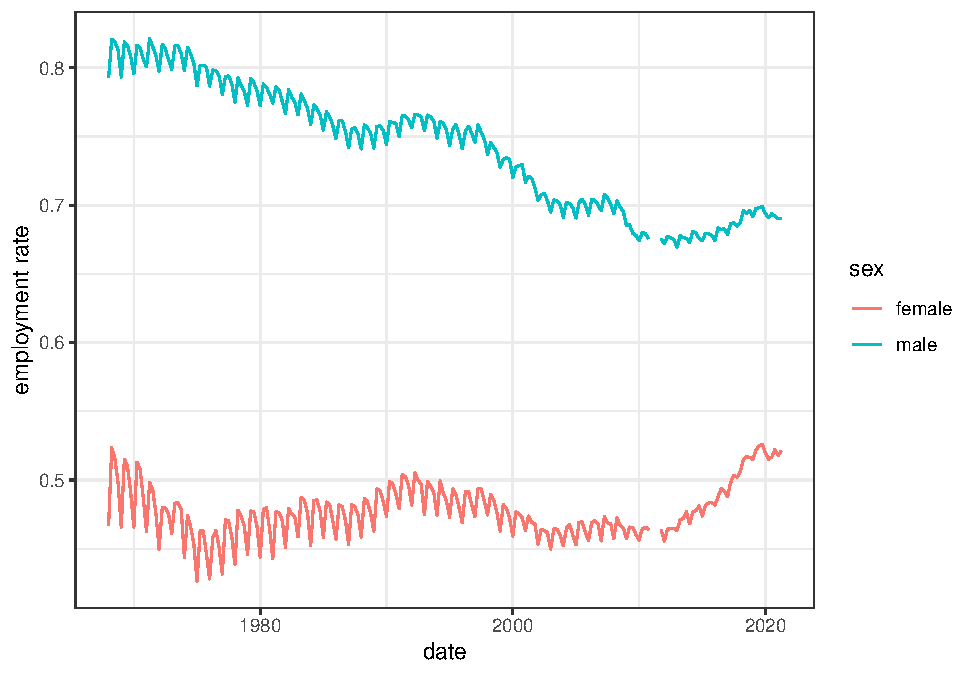
\includegraphics{CPS_Japan_files/figure-latex/unnamed-chunk-3-1.pdf}

\hypertarget{year-to-year-difference}{%
\section{Year-to-year difference}\label{year-to-year-difference}}

\begin{itemize}
\tightlist
\item
  Report change of employment rate \(\tilde e_{g,m,y}=e_{g,m,y}/e_{g,m,y-1}\)
\end{itemize}

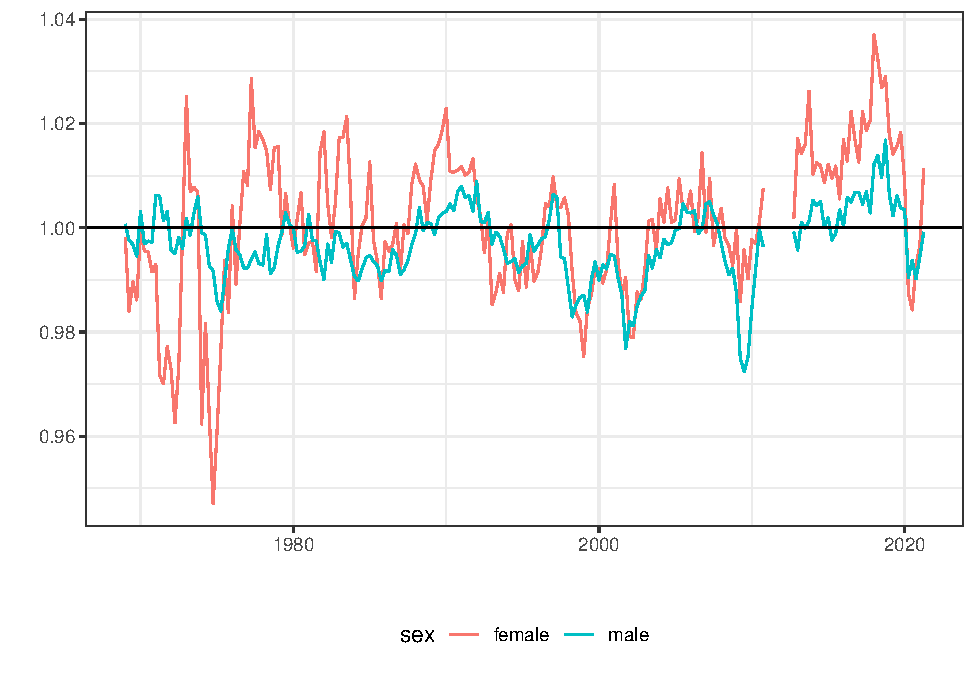
\includegraphics{CPS_Japan_files/figure-latex/y_to_y-1.pdf}

\hypertarget{gender-gap}{%
\section{Gender gap}\label{gender-gap}}

\begin{itemize}
\tightlist
\item
  Report change of employment rate \(\tilde e_{male,m,y} - \tilde e_{female,m,y}\)
\end{itemize}

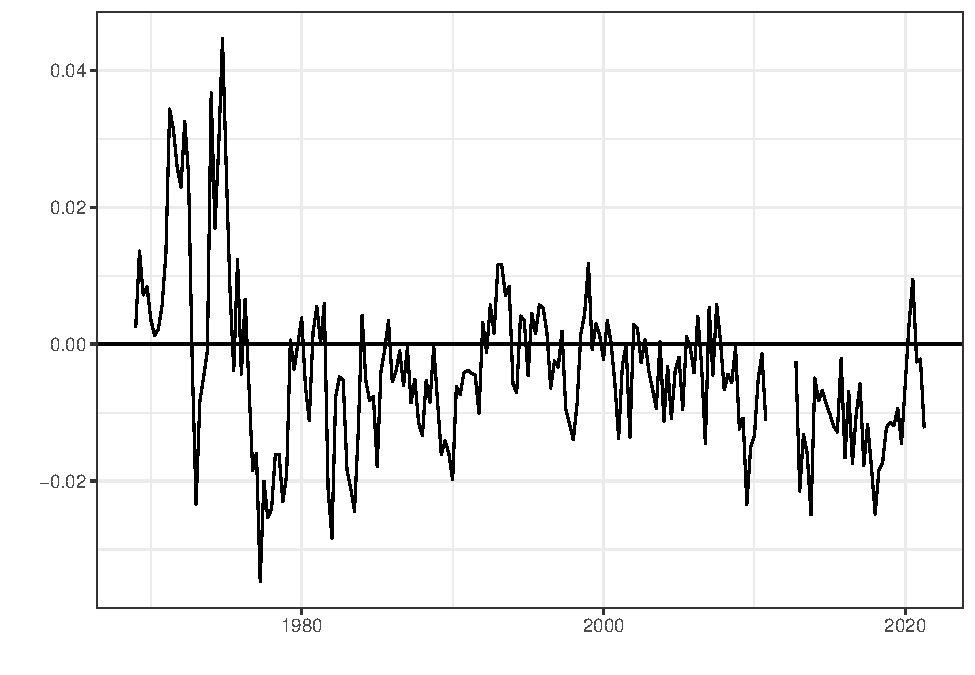
\includegraphics{CPS_Japan_files/figure-latex/unnamed-chunk-4-1.pdf}

\hypertarget{simple-description-short-run}{%
\chapter{Simple description: Short run}\label{simple-description-short-run}}

\begin{itemize}
\tightlist
\item
  Describe labor market after 2019.
\end{itemize}

\hypertarget{environment-1}{%
\section{Environment}\label{environment-1}}

\hypertarget{data-1}{%
\section{Data}\label{data-1}}

\hypertarget{employment-rate-1}{%
\section{Employment rate}\label{employment-rate-1}}

\begin{itemize}
\tightlist
\item
  Report \(e_{g,m,y} = \frac{Employment_{g,m,y}}{Population_{g,m,y}}\), where \(Employment_{g,m,y}\) and \(Population_{g,m,y}\) are numbers of employment and population over 15 years old in month \(m\), year \(y\) and gender group \(g\), respectively.
\end{itemize}

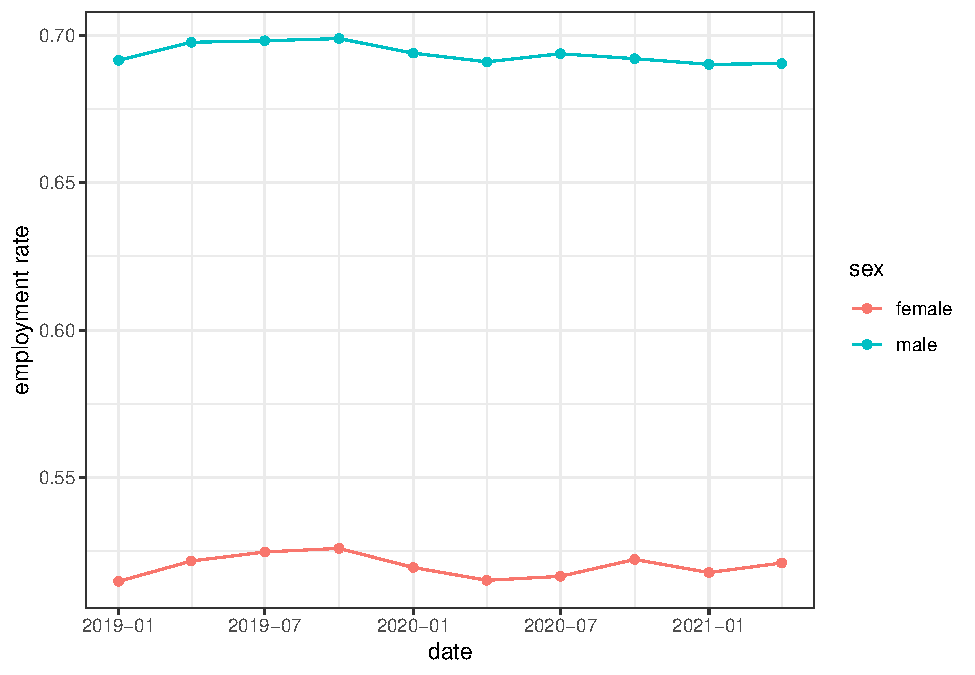
\includegraphics{CPS_Japan_files/figure-latex/unnamed-chunk-7-1.pdf}

\hypertarget{year-to-year-difference-1}{%
\section{Year-to-year difference}\label{year-to-year-difference-1}}

\begin{itemize}
\tightlist
\item
  Report change of employment rate \(\tilde e_{g,m,y}=e_{g,m,y}/e_{g,m,y-1}\)
\end{itemize}

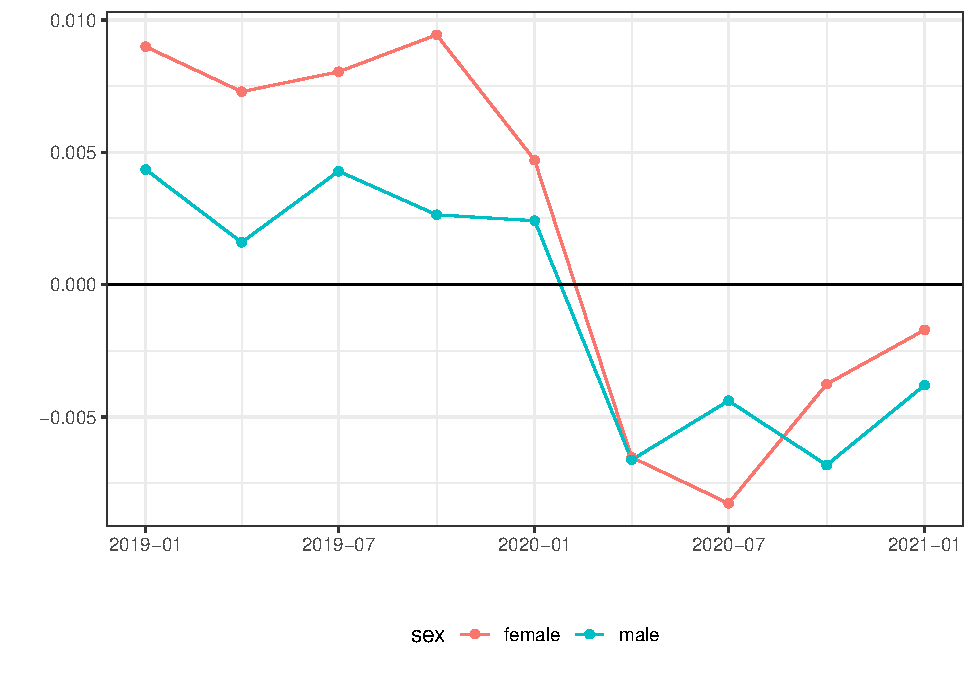
\includegraphics{CPS_Japan_files/figure-latex/unnamed-chunk-8-1.pdf}

\hypertarget{gender-gap-1}{%
\section{Gender gap}\label{gender-gap-1}}

\begin{itemize}
\tightlist
\item
  Report change of employment rate \(\tilde e_{male,m,y} - \tilde e_{female,m,y}\)
\end{itemize}

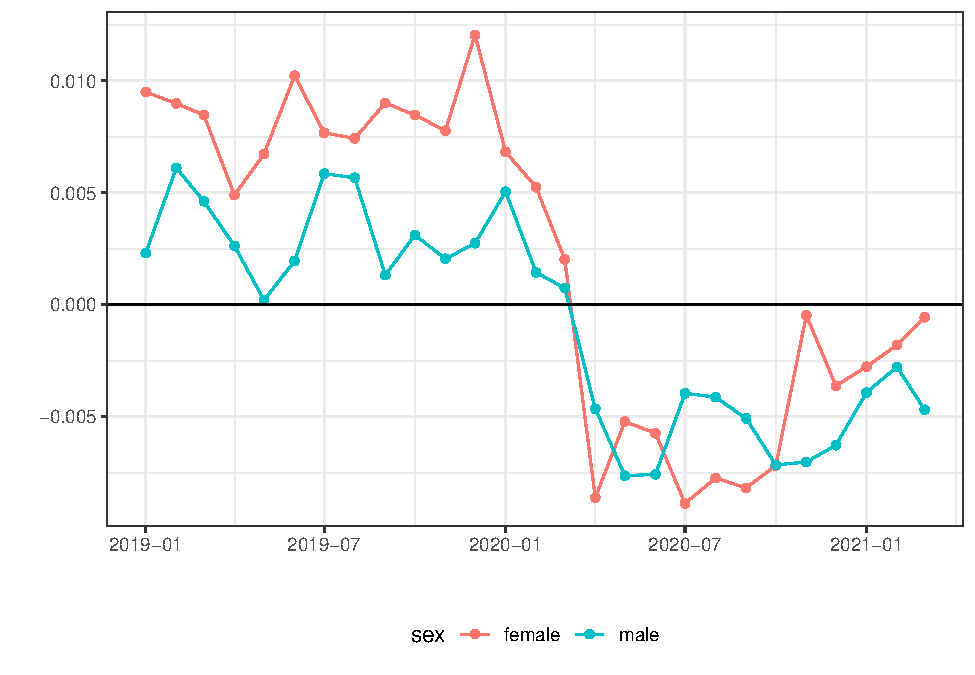
\includegraphics{CPS_Japan_files/figure-latex/unnamed-chunk-9-1.pdf}

\hypertarget{detail}{%
\chapter{Detail}\label{detail}}

\begin{itemize}
\item
  Describe labor market after 2011.
\item
  Report rates of workers who are employed primarily or partly.
\end{itemize}

\hypertarget{environment-2}{%
\section{Environment}\label{environment-2}}

\hypertarget{data-status}{%
\section{Data status}\label{data-status}}

\hypertarget{employment-rate-2}{%
\section{Employment rate}\label{employment-rate-2}}

\begin{itemize}
\tightlist
\item
  Report \(e_{g,m,y} = \frac{Employment_{g,m,y}}{Population_{g,m,y}}\), where \(Employment_{g,m,y}\) and \(Population_{g,m,y}\) are numbers of employment and population over 15 years old in month \(m\), year \(y\) and gender group \(g\), respectively.
\end{itemize}

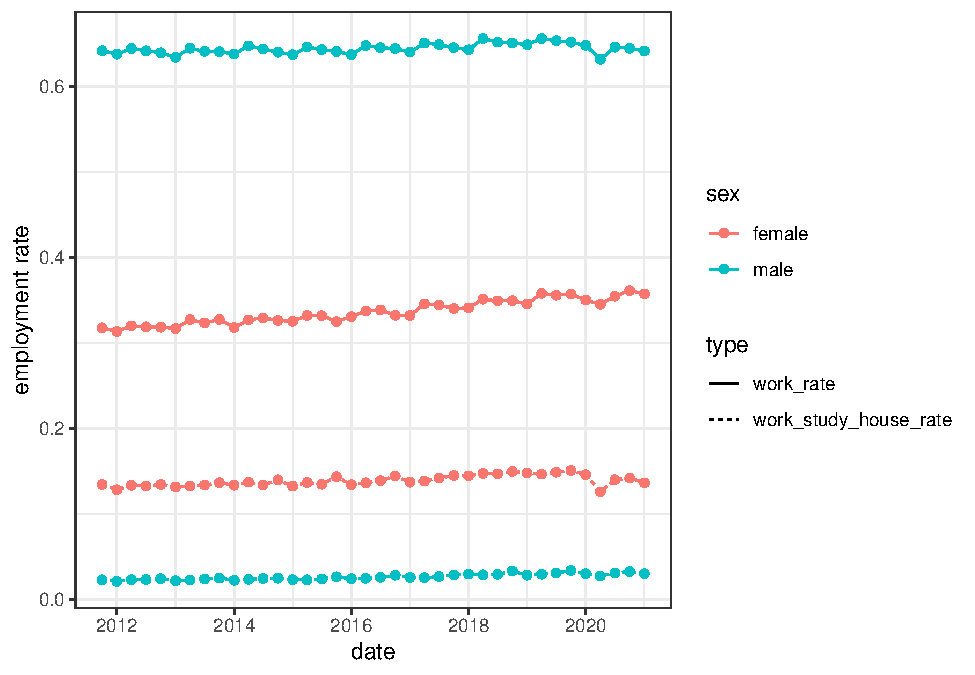
\includegraphics{CPS_Japan_files/figure-latex/unnamed-chunk-12-1.pdf}

\hypertarget{year-to-year-difference-2}{%
\section{Year-to-year difference}\label{year-to-year-difference-2}}

\begin{itemize}
\tightlist
\item
  Report change of employment rate \(\tilde e_{g,m,y}=e_{g,m,y}/e_{g,m,y-1}\)
\end{itemize}

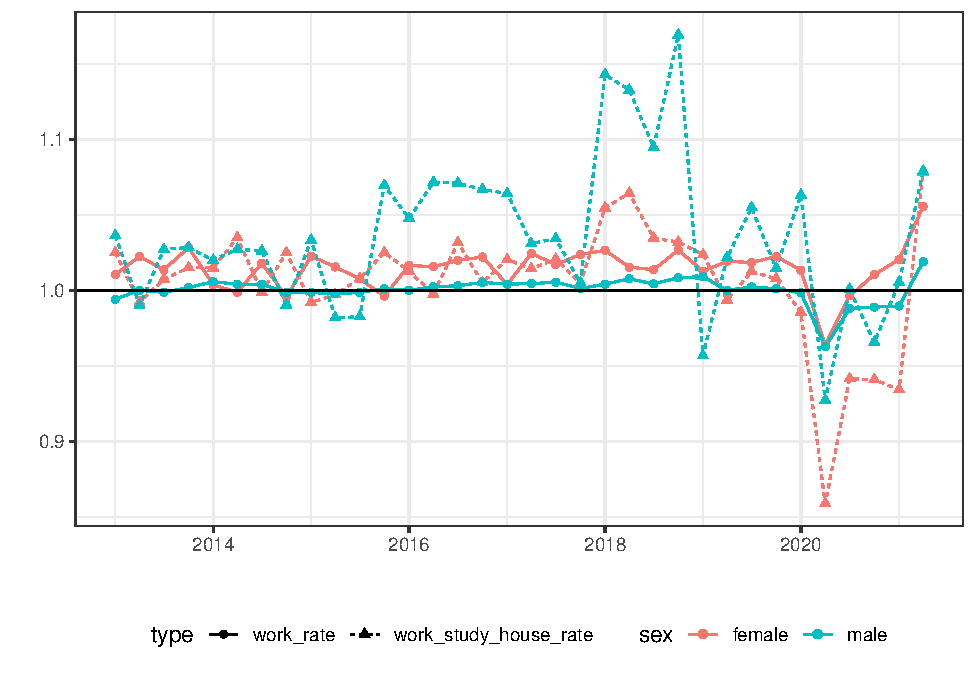
\includegraphics{CPS_Japan_files/figure-latex/unnamed-chunk-13-1.pdf}

\hypertarget{gender-gap-2}{%
\section{Gender gap}\label{gender-gap-2}}

\begin{itemize}
\tightlist
\item
  Report change of employment rate \(\tilde e_{male,m,y}-\tilde e_{female,m,y}\)
\end{itemize}

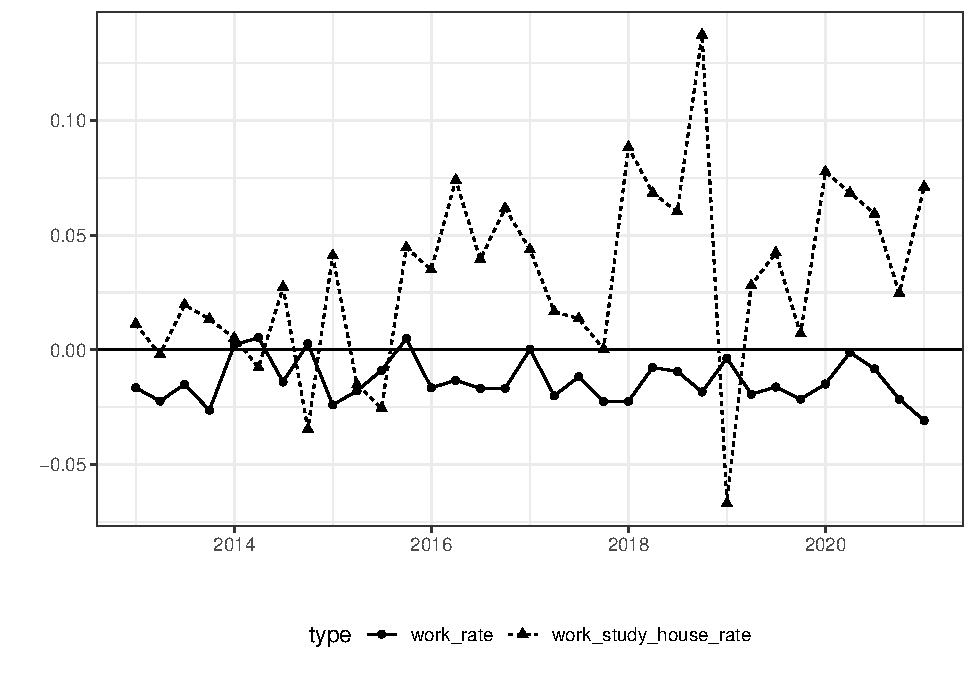
\includegraphics{CPS_Japan_files/figure-latex/unnamed-chunk-14-1.pdf}

\hypertarget{working-hour}{%
\chapter{Working hour}\label{working-hour}}

\begin{itemize}
\item
  Describe labor market after 2011.
\item
  Report working hours.
\end{itemize}

\hypertarget{environment-3}{%
\section{Environment}\label{environment-3}}

\hypertarget{data-status-1}{%
\section{Data status}\label{data-status-1}}

\hypertarget{working-hour-1}{%
\section{Working hour}\label{working-hour-1}}

\begin{itemize}
\tightlist
\item
  Report \(e_{g,m,y} = hour_{g,m,y}\), where \(hour_{g,m,y}\) is working hours.
\end{itemize}

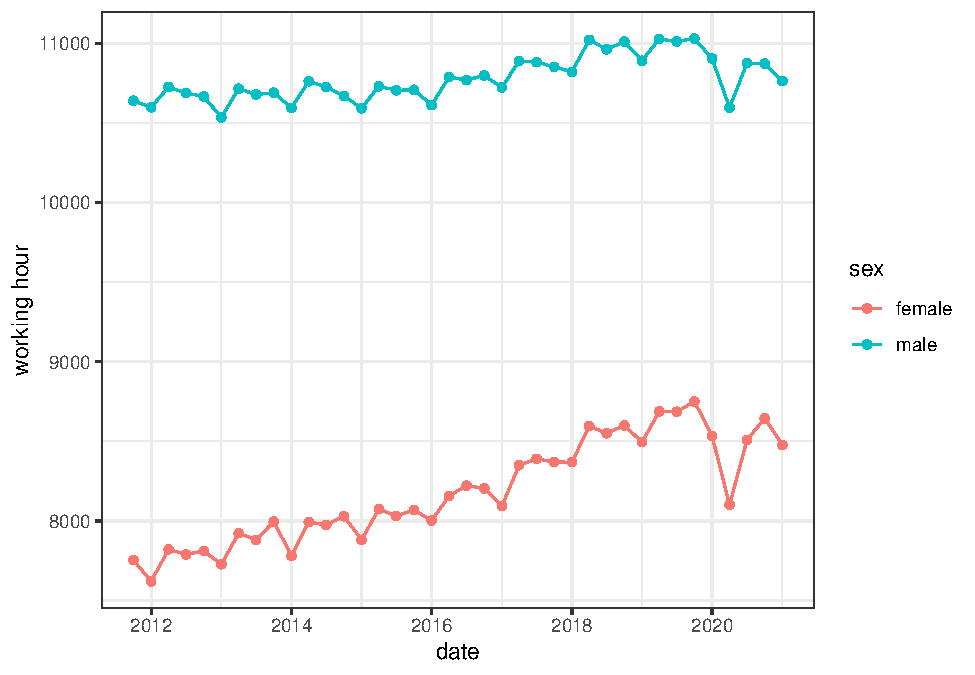
\includegraphics{CPS_Japan_files/figure-latex/unnamed-chunk-17-1.pdf}

\hypertarget{year-to-year-difference-3}{%
\section{Year-to-year difference}\label{year-to-year-difference-3}}

\begin{itemize}
\tightlist
\item
  Report change \(\tilde e_{g,m,y}=e_{g,m,y}/e_{g,m,y-1}\)
\end{itemize}

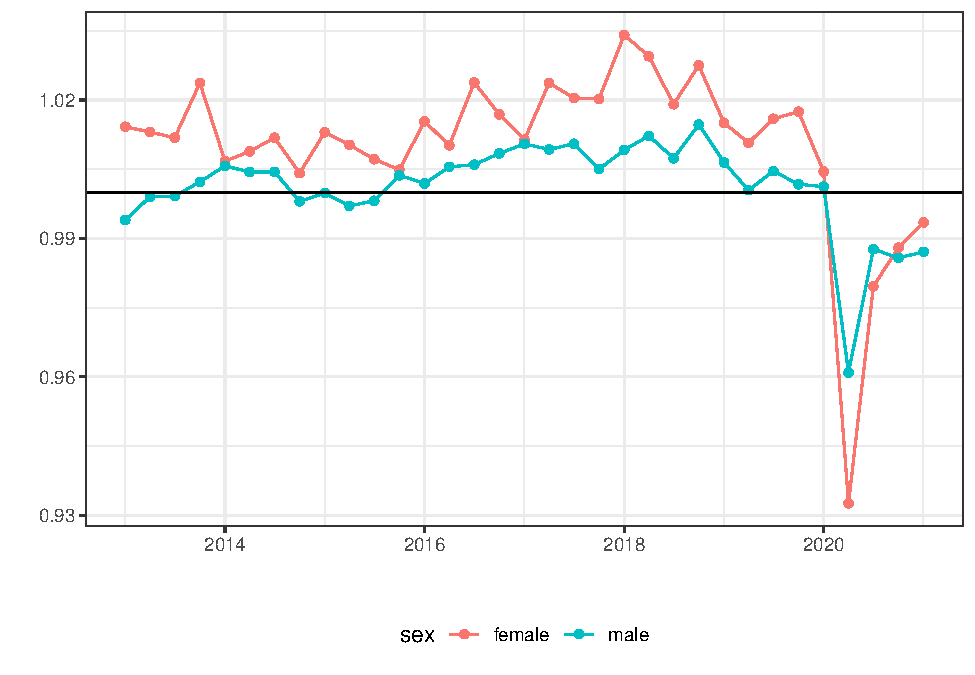
\includegraphics{CPS_Japan_files/figure-latex/unnamed-chunk-18-1.pdf}

\hypertarget{gender-gap-3}{%
\section{Gender gap}\label{gender-gap-3}}

\begin{itemize}
\tightlist
\item
  \(\tilde e_{male,m,y}-\tilde e_{female,m,y}\)
\end{itemize}

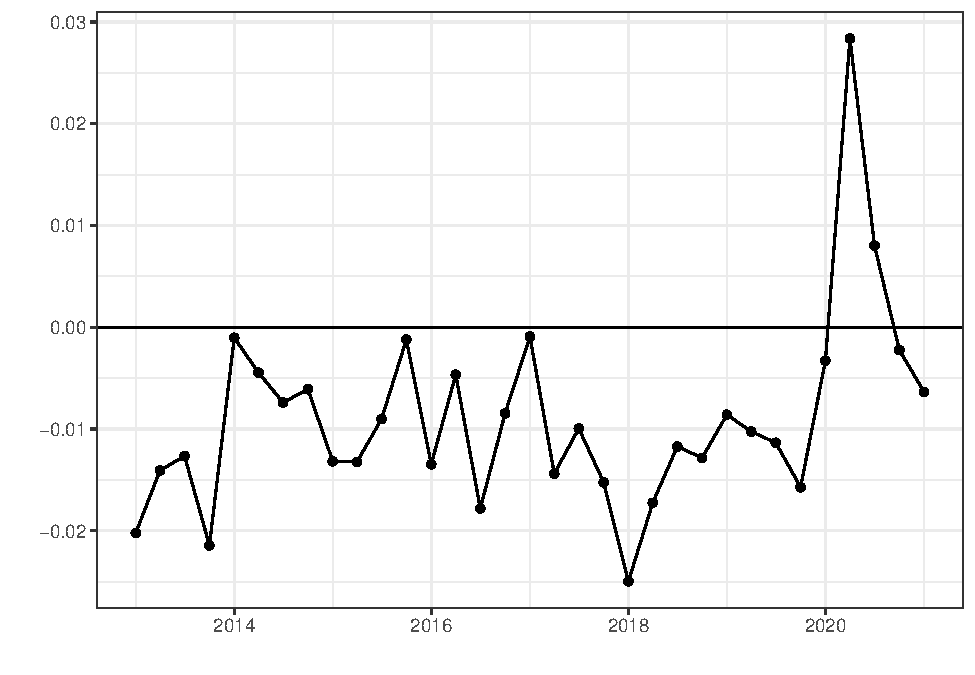
\includegraphics{CPS_Japan_files/figure-latex/unnamed-chunk-19-1.pdf}

  \bibliography{book.bib,packages.bib}

\end{document}
